\begin{event}
  {GAP--Singular School and Meeting}
  {TODO}  % {eventId}
  {PfalzAkademie, Lambrecht, Germany, 15--23 August, 2019}
  {TODO}  % {Partners (use Partners id, separated with coma)}
  {33}
  {4}  % {nb of ODK participants}
  {https://opendreamkit.org/meetings/2019-04-02-GAPSingularMeeting/}

\textbf{Main goals.}
The main goals were to finish ODK related developer tasks as well as
  to introduce beginners to \GAP and \Singular, present
computer algebra--related work, and share ideas through workshops.

\textbf{ODK implication.}
The event was fully funded by ODK. Costs are still pending due to
overseas travel claims.

\textbf{Event summary.}
The event consisted of three parts:
\begin{itemize}
\item School: a sequence of workshops to introduce beginners to \GAP, \Singular,
  and open-source development principles.
\item Mini-conference: talks to allow participants to present computer
  algebra--related work to each other.
\item Workshops: a set of workshops dedicated to specific computer algebra
  problems.
\end{itemize}

\textbf{Demographics.}
The workshop had just under 50 registered participants, not all of which
  were able to attend (VISA delays).
The participants came from more than 10 countries on 4 continents.
We had a total of 8 women attending.

\textbf{Results and impact.}
In the School, tutorials were given that introduced participants to:
\begin{itemize}
\item Best practices in software development (Max Horn);
\item Basic use of \GAP (Michael Torpey);
\item Advanced Topics in \GAP (Thomas Breuer);
\item Basic use of \Singular (Christian Eder, Andreas Steenpaß, Isabel Stenger);
\item Parallel modular algorithms in Singular (Christian Eder, Andreas Steenpaß, Isabel Stenger);
\item CAP: Categories, algorithms, programming (Sebastian Posur).
\end{itemize}
These tutorials were complemented by informal discussions, and chances for
learners to answer questions.  The ``Best practices'' and ``Basic use of \GAP''
sessions followed material from appropriate Software Carpentry courses
(\url{https://software-carpentry.org/lessons/}): ``Version Control with Git''
and ``Programming with GAP'' respectively.

The workshops of basic \Singular and \GAP were well received - several 
participants were either novices in \GAP or \Singular.
For the non-beginners, the advanced workshops on modular algorithms in 
\Singular and on CAP (a \GAP package for categories, in particular in,
but not restricted to, algebraic geometry) proved very intersting.

The next part, contributed talks, covered only a single day. However
the talks originated in  many different areas of mathematics and covered
many successful challenging applications of components (\GAP, \Singular)
of ODK.

The final part, comprised of workshops on \GAP, \Singular and CAP
allowed us to close off remaining issues with regard     
to the integration of the ODK work into the various packages, e.g.              
improvements to the integration of the fast multivariate polynomial             
arithmetic in Singular. The workshop was in particular extremely useful in      
bringing participants together to discuss some of the remaining technical       
challenges and in understanding the mathematical challenges real world          
researchers were facing and how they could be solved using tools developed      
during ODK. For example, it was discovered during the workshop that a           
bottleneck experienced by one of the participants was down to fast              
multivariate polynomial arithmetic (via rational functions) which was then      
directly worked on by participants of the meeting. There was also a project     
to improve integration of \Singular into the Singular.jl
 subsystem of the        
Oscar computer algebra system specifically so that Gr\"{o}ber bases could       
be computed over coefficient fields implemented by ODK components. This         
project was finalized and merged at the workshop after months of                
unsuccessful previous attempts.

The \GAP workshop was part of the \GAP 4.11 release process which is critical
for the dissemination of ODK components such as \libGAP. At the workshop,
changes to the \libGAP system were documented and significant progress was
made towards rapping up the release to reach users. This included
dissemination of \GAP into the Debian distribution. There were also lively
discussions about the \GAP-\Jupyter integration.


\begin{figure}[ht]
  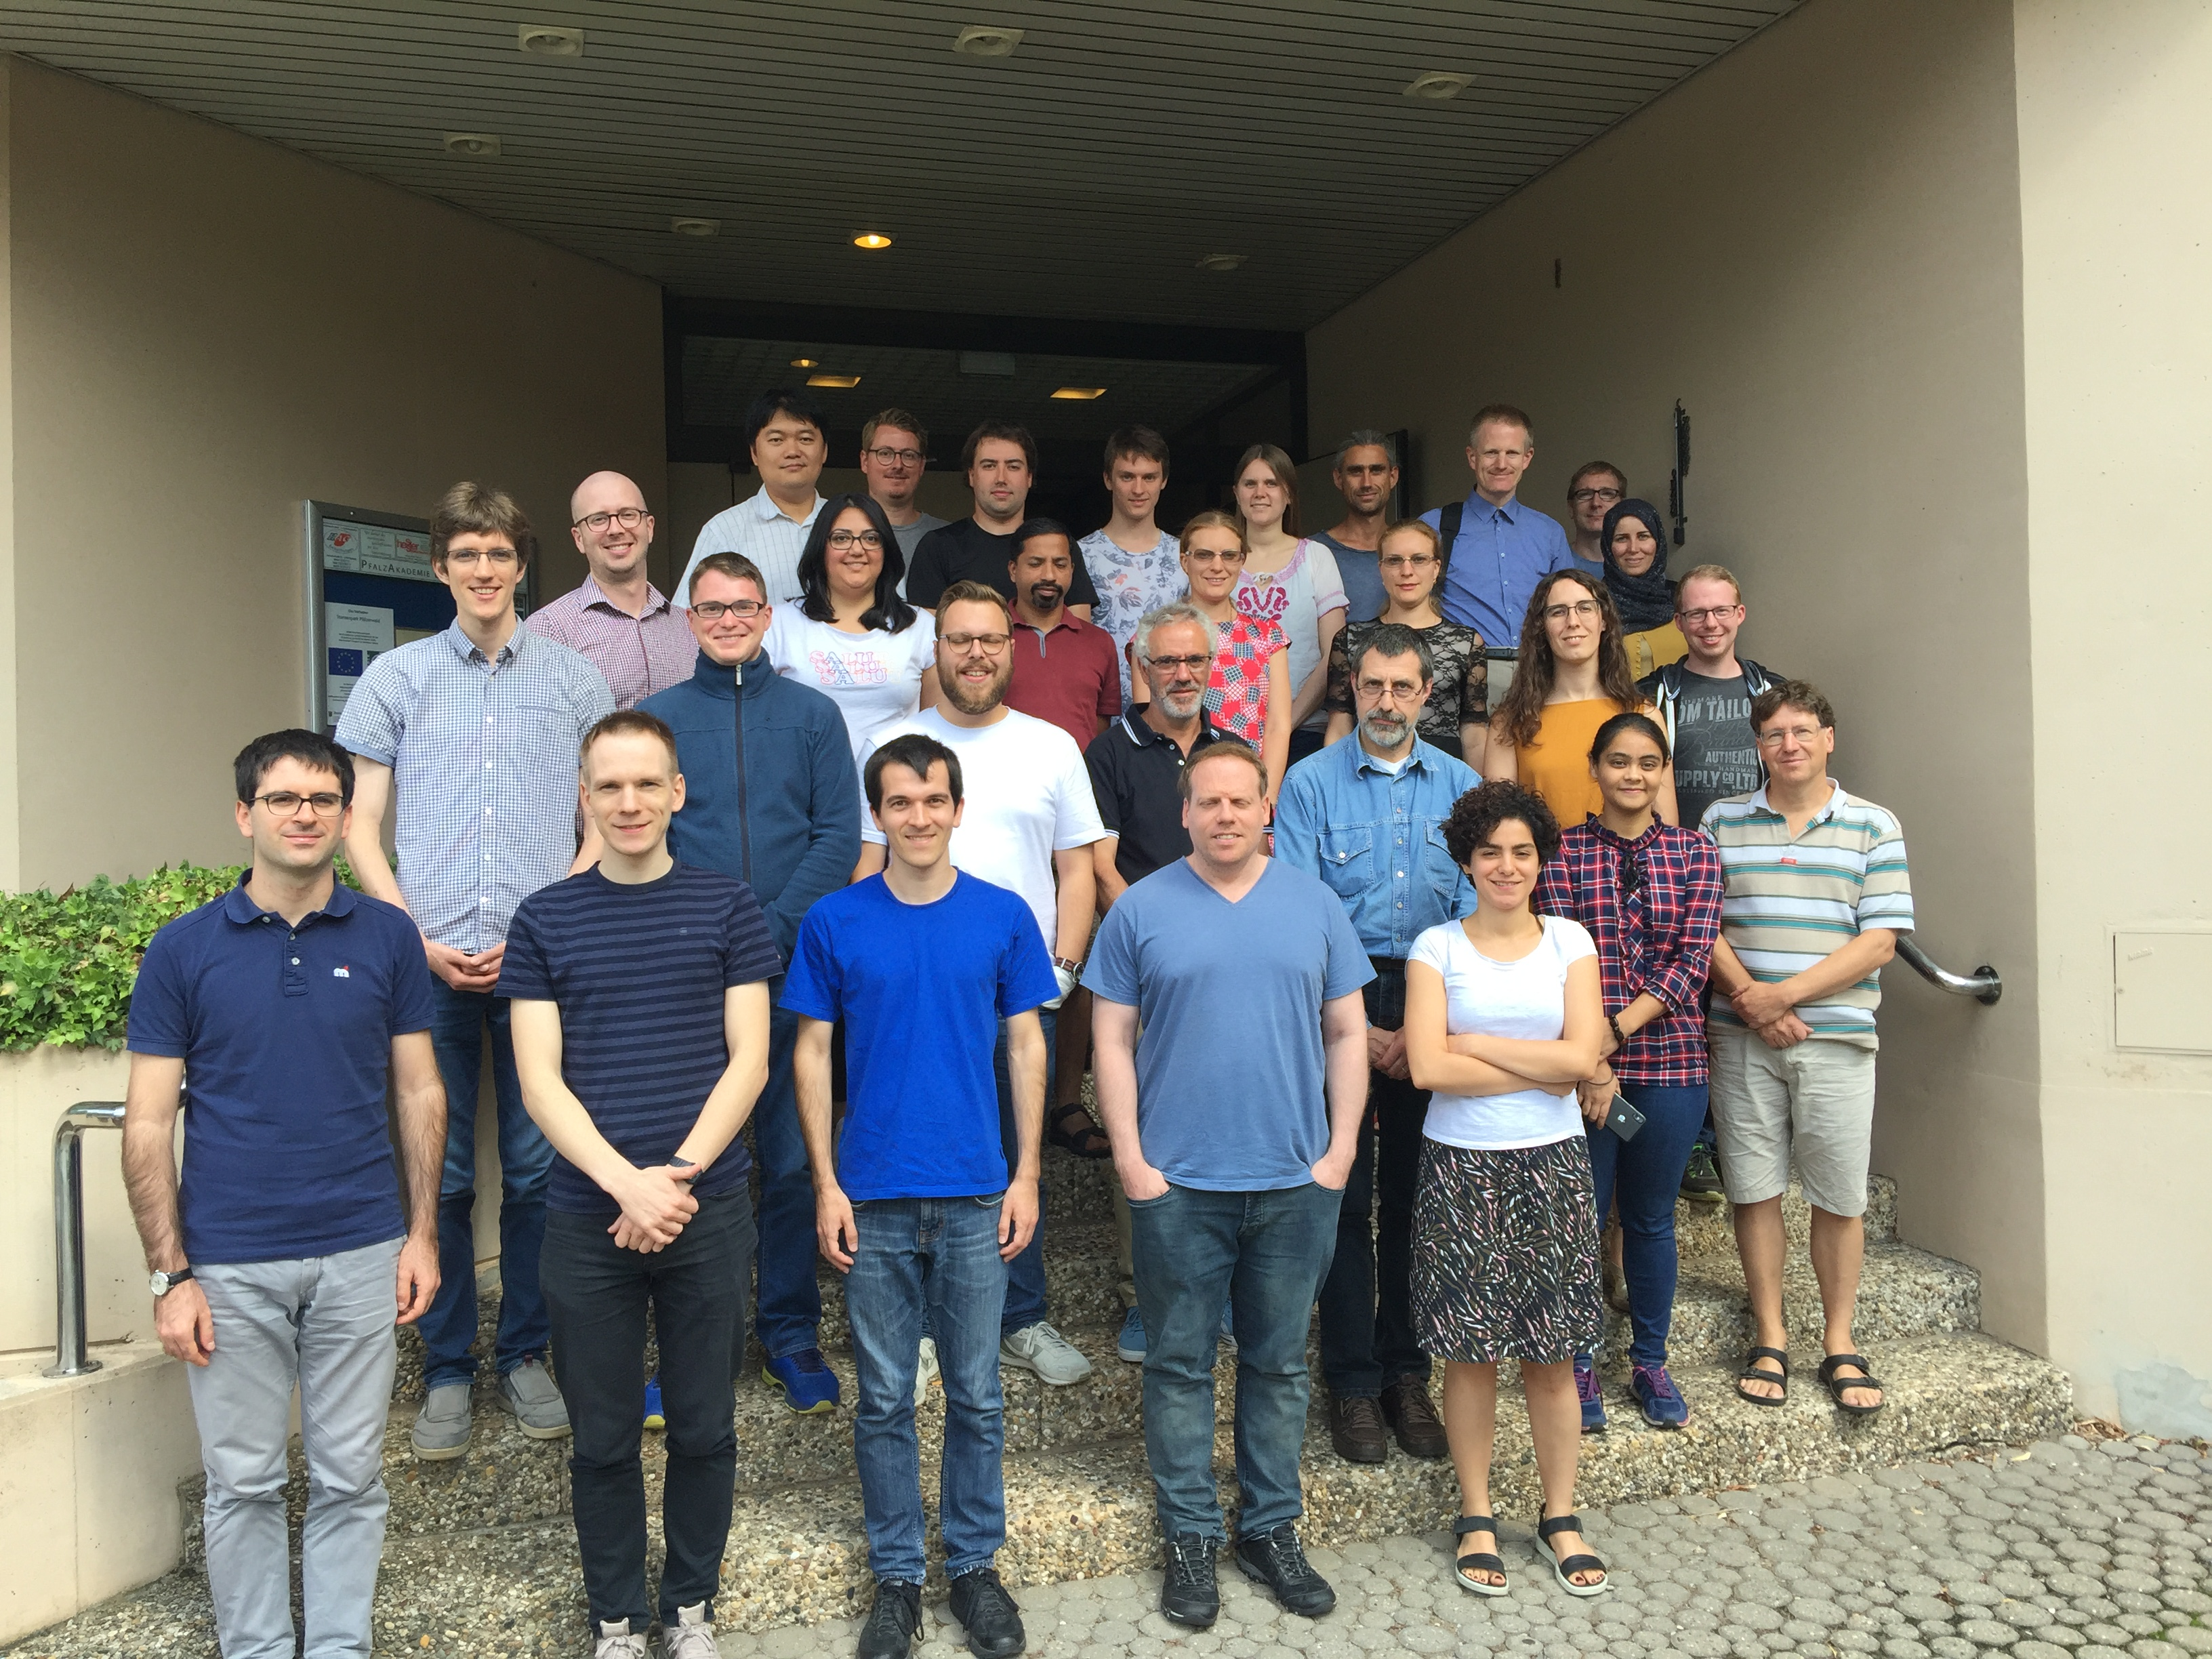
\includegraphics[width=\textwidth]{gap-singular-participants}
  \caption*{Conference photo of GAP--Singular meeting}
\end{figure}

\end{event}
